%\newpage
\section{Algorytm sterowania}

Algorytm sterowania pojazdem w sieci miejskiej składa się w ogólności z 3 części:

\begin{itemize}
	\item 
	Wybór \textit{trasy} (route planning) -- polega na wyborze kolejnych dróg, skrzyżowań etc. po~których będzie poruszał się pojazd przemieszczający się z punktu A do B. Jest to równoznaczne z~wyborem kolejnych wierzchołków i krawędzi w grafie. Np. autostrada A2 jest \textit{trasą}, którą można przejechać z Warszawy do Poznania. 
	\item 
	Wybór \textit{trajektorii} (path planning) -- polega na wyborze pewnej krzywej, po której pojazd ma się poruszać w ramach \textit{trasy}. Np. jest to \textit{krzywa}, po której porusza się samochód skręcający na skrzyżowaniu.
	\item 
	Wybór \textit{sterowań} pojazdu -- polega na zadaniu pojazdowi skrętu kół i prędkości tak żeby w~odpowiedni sposób poruszał się po trajektorii i reagował na zmieniające się otoczenie (np. nagłe hamowanie w momencie wykrycia przeszkody).
\end{itemize}

Kierując się powyższym podziałem zaprojektowano strategię sterowania mającą dwa główne cele: zapewnienie bezpiecznego i bezkolizyjnego przejazdu, a także minimalizację czasów poszczególnych przejazdów. W celu uproszczenia strategi (ale bez straty ogólności) przyjęto następujące założenia:

\begin{itemize}
	\item 
	Sieć dróg reprezentowana jest przez graf skierowany z ważonym krawędziami.	
	\item 
	Pojazd może zmienić kierunek jazdy tylko w momencie dojeżdżania do węzła grafu (skrzyżowania). Dopuszczalne są: zawracanie, skręt i jazda prosto 
	\item 
	Pierwszeństwo na węźle określane jest na podstawie znaków, sygnalizacji, priorytetów dróg etc.
	\item 
	Samochody posiadają pełną wiedzę o sieci dróg oraz występujących na nich ograniczeniach prędkości.
	\item 
	Wszystkie drogi mają co najwyżej jeden pas w każdym kierunku.
	\item 
	Decyzję o zmianie trasy (route) samochody podejmują	w momencie dojazdu do węzła.
	\item
	Pojazdy dysponują pełna wiedzą o stanie (liczbie i prędkościach pojazdów) na drogach wychodzących ze skrzyżowania do którego się zbliżają. Na tej podstawie mogą lokalnie aktualizować wagi krawędzi we własnym grafie dróg. W rzeczywistym świecie możliwe jest bowiem określenie zakorkowania najbliższych dróg "na oko".
	
\end{itemize}

\noindent W kolejnych podsekcjach szczegółowo przedstawiono kolejne części strategii sterowania.

\subsection{Wybór trasy}

Wybór trasy polega na znalezieniu najkrótszej ścieżki w grafie ważonym - stosuje się do tego np. funkcję \textit{shortestpath} w Matlabie. Przetestowane i porównane zostaną 3 strategie doboru wag w grafie. W pierwszym, najprostszym przypadku wagi krawędzi $w_i$ są równe długości dróg $l_i$:

\begin{equation}
w_i = l_i
\end{equation}

W drugim przypadku wagi niosą również informację o maksymalnej dopuszczalnej prędkości na drodze $v_{i,MAX}$ - są równe minimalnemu dopuszczalnemu czasowi przejazdu:

\begin{equation}
w_i = \frac{l_i}{v_{i,MAX}}
\end{equation}

Trzeci przypadek jest rozszerzeniem przypadku drugiego. Dla każdego samochodu, wagi krawędzi wychodzących z węzła do którego pojazd się kieruje, są zaktualizowano o informację na~temat średniej prędkości przejazdu $v_{i,avg}$ samochodów po danej krawędzi - pojazd rozszerza swoją wiedzę o pewną obserwację otoczenia (korków). Wszystkie pozostałe krawędzie przyjmują wagi jak w przypadku drugim:

\begin{equation}
w_i = \frac{l_i}{v_{i,avg}}
\end{equation}

Trzeci przypadek można rozszerzyć o jakąś formę pamięci pojazdu o dotychczas miniętych krawędziach. Decyzja o zmianie trasy podejmowana jest za każdym razem gdy pojazd zbliża się do węzła.

\begin{figure}[!h]
\centering
	\centering
	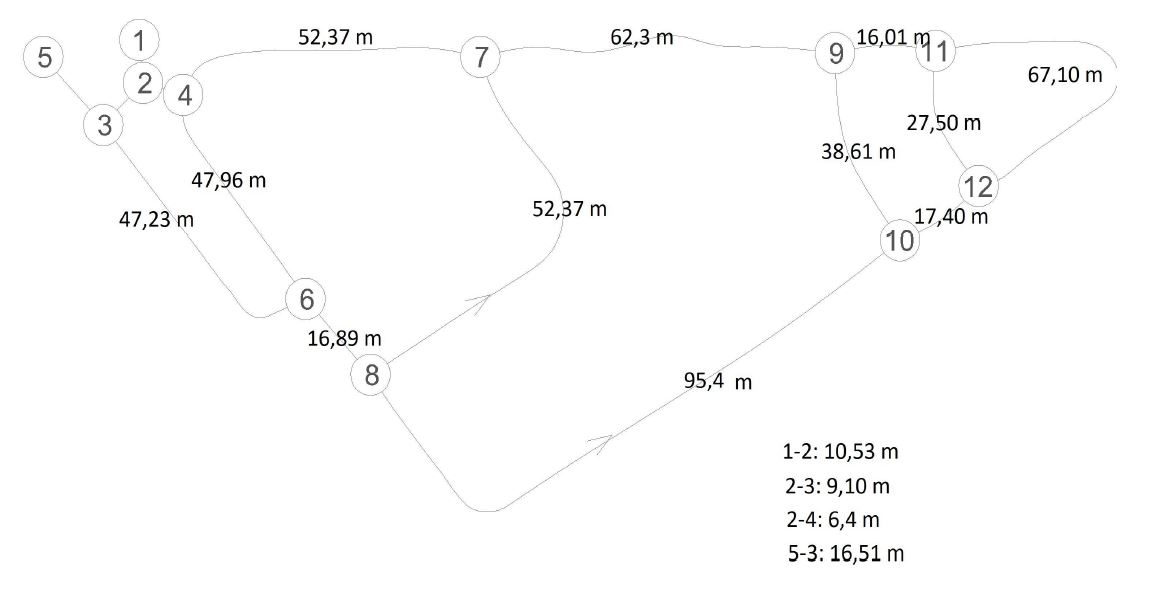
\includegraphics[width=.8\linewidth]{graf.jpg}
	\caption{Przykładowy graf reprezentujący sieć dróg, źródło: A. Barsi et al. An offline path planning method for autonomous vehicles}
	\label{fig:graf}
\end{figure}

\subsection{Wybór trajektorii}

Trajektorie generowane będą przy pomocy funkcji \textit{pathplannerRRT} i \textit{smoothpathspline} w~Matlabie. Do tych funkcji przesyłane będą informację o aktualnej trasie, mapie dróg, a także informację z czujników wykrywających przeszkody (inne pojazdy). Na wyjściu funkcje generują pewną krzywą.

\begin{figure}[!h]
	\centering
	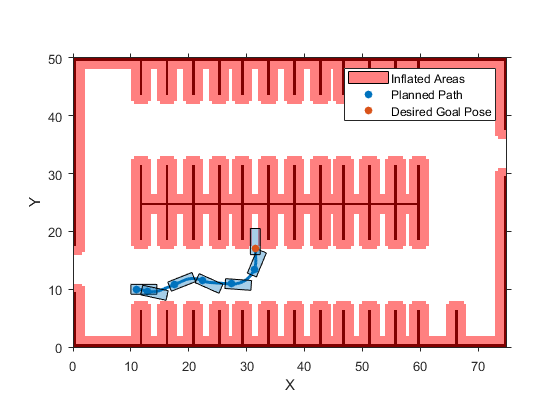
\includegraphics[width=.8\linewidth]{trajektoria.png}
	\caption{Przykładowa trajektoria wygenerowana w programie Matlab, źródło: Mathworks.com.}
	\label{fig:trajektoria}
\end{figure}

\subsection{Wybór sterowań}

Na podstawie wygenerowanej w poprzednim kroku krzywej, korzystając z funkcji \textit{lateralControllerStanley} przyjmującej trajektorię, wygenerowany zostanie skręt kół. Prędkość pojazdu będzie zadawana pewną logiką biorącą pod uwagę znaki drogowe, sygnalizacje świetlną, a także obecność innych pojazdów - ochrona przed kolizją. Wybrany skręt oraz prędkość wysyłane będą do~symulatora V-REP.
 
